\chapter{Background}
\label{background}
\epigraph{
In order to agree to talk, we just have to agree we are talking about roughly the same thing.
}
{\textit{The Feynman Lectures on Physics, Motion, Richard Feynman, 1961.}}

%%%What is Software Evolution
Software evolution is the process of change made to a software system to maintain it, or to extend its functionality over the systems lifetime.
This evolution is required in order to adapt the system to the software environment, accommodate new user requirements, fix errors, or prevent errors from occurring.
Evolving software can be difficult as there is a chance of introducing new errors, and the more the system evolves the more complex it can become.
Software evolution is also costly, as can be seen with the example of the Y2K bug, where it has been estimated that over \$300 billion was spent fixing software in anticipation for the year 2000.
%TODO cite

%%%Component Evolution
Creating software from encapsulated units, called software components, can help mitigate negative effects of the software evolution process.
Originially software components where defined in order to maximise reuse to help lower costs of producing software. 
Software is then created from composing together many software components in a manner specified by a \textbf{component model}.
The component model is the specification of how software components are described and how they relate to each other to form the system.

%%%Broken into two parts
The evolution of a component based software can be broken into two different cycles: the evolution of the component, and the evolution of a component system. 
A component evolves like a typical software system, where a unit is developed, versioned then released.
However, component system evolution involves changing the system at a higher granularity, by adding and removing components.
In addition a component is usually evolved by a developer, while a component system can be evolved by a user or stakeholder of the system.
This makes the evolution of a component system significantly different from the evolution of an individual component.

%%%What is CDR
The act of evolving a component system can be difficult given the complex relationships between components.
These relationships create constraints that must be satisfied in order for the systems components to be functional.
If these relationships are explicitly defined, the satisfaction of these constraints can be automated through a function called component dependency resolution (CDR).
CDR is a powerful tool to evolve a component system.

%%%Using CDR within an evolution strategy
Another difficulty in evolving a component system arises because of the different objectives that can be aimed for.
For example, a stakeholder may wish to alter very little to minimise the risk of change, or to change as much as necessary to lower the risk of being out of date.  
These objectives are taken into account and enacted in an evolution strategy, the plan employed by the stakeholder to change and adapt their system.

%%%Defining components
How ``software component'' is defined will impact the meaning of component system evolution.
The definition of ``software component'' has not yet been specified due to community disagreements over even fundamental aspects of software components \citep{Meyer1999,Szyperski2000a, Szyperski2000, Meyer2000}.
This makes it impossible to find a definition to satisfy everyone.
By defining a software component only with respect to component system evolution, this process can be studied without the paralysis of finding a precise and complete definition.
This method may produce a definition that conflicts with others, 
though it allows this research to ignore potentially superfluous arguments.

%%%Examples of component models
With respect to component system evolution, various component models can be described.
These component models can differ by functionality, platform, or their objectives for being created.
They may also have their own CDR implementations, created to assist in their component systems evolution. 

%%%In this chapter\ldots
In this chapter, software evolution, component evolution and component system evolution are discussed and compared in section \ref{background.evolution}.
This section includes descriptions of component dependency resolution and the evolution strategies of stakeholders.
The definition of software components and component models with respect to component system evolution is then presented in section \ref{background.components}.
To conclude this chapter  examples of various component models and CDR implementation are then given in section \ref{background.models}.
This includes an introduction to the Debian model, and CUDF model that are described in more detail in the following chapters.

\section{Software Evolution and Component-Based Software Engineering}
\label{background.evolution}
Software evolution
\footnote{Sometimes also called software maintenance in this research. 
However, ``evolution'' is preferred because it implies change, where maintenance implies the restoration to a previous condition.} 
is the necessary process of changing a system to adapt the environment it exists in.
This process was first identified by \cite{Lehman1969}\footnote{though it was not refereed to as evolution at that time} 
That year \cite{McIlroy1969} also described the ideals of software components, which where an industrialised industry creating interchangeable, modular software.
This was an extension of an idea that McIlroy expressed in a memo \citep{mcilroy1964pipes} where software should be like a garden hose assemble, and components should be screwed together.

Both these domains of software engineering, software evolution and component-based software engineering, have seen massive advancement since 1969.
In this section these advancements are briefly described, leading up to the 

\subsection{Software Evolution}
\cite{Brooks1975} stated that over 90\% of the cost of a system occurs after deployment, in the software maintenance phase.
He also stated that any successful piece of software will inevitably be maintained.
This realisation lead researches to study this process of changing software after it has been released.
Arguably the core studies of software evolutions main advancement came 

%%%Software Evolution is


%%%The nature of this evolution has been explored and laws found
The nature and fundamental laws of software evolution have be explored through empirical study of the software being evolved.
By observing the evolutionary development of many software systems and analysing the results, laws, similar to the laws of nature like gravity, can be identified.
Some of the discovered laws of this evolution are outlined by \citep{lehman1980} and \citep{lehman1997}, and presented here:

\begin{enumerate}
  \item \textit{Continuing Change:} Systems\footnote{E-type systems: software implemented in a real-world computing context} must be continually adapted 
  otherwise, they become progressively less satisfactory
  \item \textit{Increasing Complexity:} As the system evolves its complexity increases unless work is done to reduce it
  \item \textit{Self Regulation:} The system evolves with statistically determinable trends and invariences
  \item \textit{Conservation of Organisational Stability:} The average effective activity rate to evolve a system is invariant over its lifetime
  \item \textit{Conservation of Familiarity:} As the system evolves, its incremental growth remains invariant to ensure users maintain mastery over the system.
  \item \textit{Continuing Growth:} The system must continually grow to maintain user satisfaction
  \item \textit{Declining Quality:} The quality of the system will decline unless rigorously maintained
  \item \textit{Feedback System:} The function a system performs is changed by the effect it has on its environment.
\end{enumerate}

%%%These laws describe the fact that it is impossible to create a single satisfactory system, and an iterative approach is best to strive for continual satisfaction
These laws make the software engineer's objective of creating a satisfactory system impossible, as they are chasing a moving target.
A software engineer's goal is then to continually change a system to make it more satisfactory, with minimal cost and delay \citep{Lehman2006}.
This change must be accomplished while the engineer maintains intellectual control over the complexity of the system \citep{Brooks1975}, 
as the more complex a system, the greater the difficulty to change it.

This iterative process can be seen in the spiral model shown in figure \ref{spiral}, first presented by \citep{Boehm1988}.
This shows the tasks of communication, planning, modeling, construction, and deployment iteratively completed in order to create a software system.
\begin{figure}[h!]
\begin{center}
  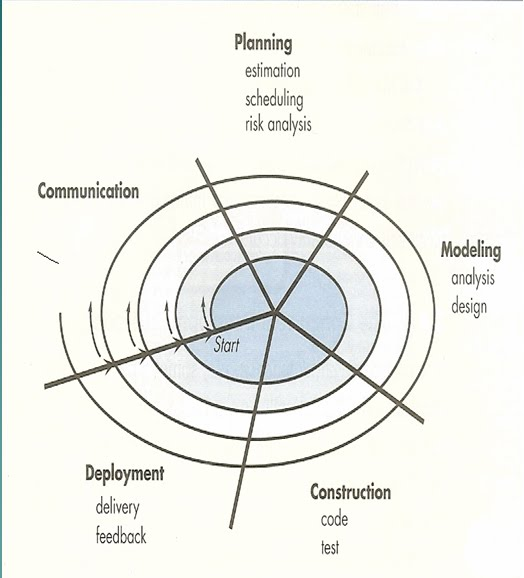
\includegraphics[width=0.6\textwidth]{backgroundpics/spiral}
  \caption{The spiral software model}
  \label{spiral}
\end{center}
\end{figure}

%%%Figure of the iterative spiral development cycle showing its mitigation of the negative effects of the laws of software evolution
This figure shows the evolutionary cycle of software development through the stages of communication, planning, modeling, construction and deployment.
These stages are continually iterated  until the software project reaches the end of its life. 
This is a common model used to develop a software system, and shows the necessity to consider evolution during the software development.  

%%%Therefore a software engineer, must\ldots
A software engineer must create a system that can be quickly altered to adapt to a changing environment, 
while working to reduce the inevitable complexity caused by this change.

\subsection{Component-Based Software Evolution}
%%%How CBSE helps with these goals of a software developer
As stated above, the goals of a software engineer are to create a system that can be continually changed with minimal cost and delay,
while maintaining intellectual control over the systems complexity.
Towards these goals component based software engineering (CBSE) was created.

%%%What is component based software engineering
CBSE is considered by some to be the future for development of software systems \citep{Szyperski2002}.
It creates software systems by composing encapsulated units, software components, together.
The encapsulation of software components limits the relationships to one another, decreasing complexity and increasing intellectual control over the system.
Using software components also has the benefit of encouraging reuse, where a component developed for one system can be used in others easily.

%%%Complexity in a monolithic system vs change to component system
In a non-component based system any part of the system can depend on any other part.
This can create unnecessary complexity which makes evolving the system a difficult task.
This problem has lead to metrics \citep{martin2003} to measure the complexity of dependencies to try to mitigate their effect on the system.
Software components should be encapsulated except for purposely exposed interfaces that can be used by other components.
Limiting relationships to either between components or interfaces is intended to reduce the complexity of the system.
This reduced complexity can lower the difficulty of change to the system, making evolution less costly.
Metrics \citep{Chen2011} developed that use the relationships of component system can be employed to help further reduce complexity.

%%%Intellectual control over the complexity of the system is increased
The reduction of the complexity in component based system has the additional benefit of increasing the intellectual control over a system.
That is, a developer can grasp concepts and relationships between components easier than between finer grained units like objects.
This lower complexity should allow the developer to make more effective changes to the system 
as the number of elements and their relationships are decreased.

%%%Maximising reuse
Reuse is often cited as the main driving force of component technology as it has been empirically shown to increase the quality and productivity within software development \citep{hallsteinsen_experiences_1997}.
The amount of reuse in a system will also decrease the amount of necessary change during system evolution, as there is less replicated functionality to maintain.
The greatest obstacle to reuse is the difficultly to locate and access required functionality quickly and easily \citep{Ye2001}.
As a component expresses the functionality it provides in the interfaces it exposes, the ability to find and reuse functionality is increased.

%%%Conclusion
An important distinction must now be made between the evolution of a single component, and the evolution of a component system.
This discussion is continued in the following section.

\subsection{Component Evolution vs. Component System Evolution}
%%%Evolution of a component system is made up of two cycles, the component evolution and system evolution.
Evolution is the repeated change of a software system to adapt to its context.
There are two contexts that exist when considering the evolution of a component based system:
the context the component exists in, and the context that the component system exists in.
These two contexts may be distinct and cause two different cycles of evolution, the evolution of individual components, and the evolution of component systems.
For each of these contexts there exists a separate process of evolution.
These processes, although related, have different features and aspects that must be discussed.

\subsubsection{Component Evolution}
%%%Two main differences with component evolution and typical software evolution, is the definition and testing of relationships,
%%%And the declaration and distribution of a version, not a system
The evolution of a component is similar to the evolution of a typical piece of software, using process like the one presented in figure \ref{spiral}.
The differences between component evolution and typical software evolution are caused by the encapsulation from other components and their composition into a single system.

Component encapsulation allows the simultaneous and separate development of components.
As a developer of a component may not have control over the development of related components, each component may have a different evolution cycle.
As the evolution cycle of a component will determine releases and changes to the component, this will effect other components.
Therefore the evolution of component must also consider evolution of other components that it relates to.
For example, if a component $a$ is changed, and component $b$ uses $a$'s functionality, this change may effect $b$.
As the developers of $a$ do not have control over the development of $b$, the changes must be discussed, and co-ordinated to ensure that they are not detrimental to either component.

Given a set of components, a combinatorial amount of systems could be created.
Therefore, ensuring the correctness of every possible composition could be impractical.
This means a component system relies far more on the specification of the relationships between components.
Compared to a typical piece of software, which is bundled together before deployment, only one system must be tested.

Without such encapsulation of components the testing of component systems would not be feasible.
For example, given a text editor component depends on three versions of a spell checker, 
and four versions of a font component.
There are twelve different systems that include one text editor, one spell checker and one font component.
If each of the spell checker components provided differs in functionality, the text editor would have to be tested to work with each.
Or if the font component effected the spell checker, the text editor component would have to be tested to work in all twelve systems.
By ensuring that each component follows a specification and only effect components that they relate to the combinatorial testing of systems is not necessary.
This therefore constrains the evolution of components, to ensure that they will work in different systems.

This nature of component evolution is explored in studies such as \citep{vasa2007patterns}, 
where the evolution of five components is empirically studied for patterns of evolution.
Other studies look at aspects like the evolution of specifications \citep{Mencl2001}, the models used to version components \citep{Stuckenholz2005},
and the general concepts related to this evolution \citep{Rhode2000}.
This area is closely related to the well studied and active research area of software evolution.

\subsubsection{Component System Evolution}
The evolution of a component system is accomplished through altering the set of components contained within the component system.
This is opposed to the evolution of individual component which alters the internal structure of a component.
This architectural level view of evolution is different as it does not concern itself with the internals of the constituent components only the relationships between the components.

The core functions to evolve a component system are \textbf{install} and \textbf{remove}, these add or remove a component to or from the system.
The additional function of \textbf{upgrade} can also be defined to remove then install a higher version of the same component. 
These functions are intended to be invoked by users, or other non-technical stakeholders to evolve the system,
as opposed to component evolution, which is caused by developers.
This evolution is difficult to measure as there is no way to measure the ``version'' of a component system.
 
%%%Users and other non technical stakeholders can alter the system
As the evolution is more coarsely grained than that of the evolution of a single component, the necessary technological knowledge is lowered.
To evolve a single component requires programming and software development knowledge to accomplish.
However, the evolution of a piece of software from a higher level only requires some knowledge of the component model and tools to change it.
The overhead for learning the basics of the component model and the tools to evolve has a low overhead, and can be conveyed quickly.
For example, to upgrade the components in a Debian GNU/Linux component system, the command \verb+apt-get upgrade+ is all that is needed to be executed.
To extend the system to install a component \verb+comp+ the command \verb+apt-get install comp+ can be executed.
This gives the power to evolve a system to a user.

%%%There is no version, or single metric, to describe the system state
The state a component or piece of software as it is evolved can be represented by a single measurement, a version.
The state of a component system cannot be measured with a single metric, as it is represented by a configuration of components with various versions.
A component system then forms something like a partially ordered set, where it may be impossible to determine if a system is more or less evolved than another.
For instance, a system that has version 1 of component $a$ and version 2 of component $b$, is neither more or less evolved than a system with version 2 of $a$ and version 1 of $b$.
This complexity makes it difficult to compare systems, and make decisions about actions to be taken.

This process of component system evolution is empirically studied in \citep{fortuna2011} by looking at the first ten releases of the Debian Linux/GNU distribution,
and using graph metrics to analyse the evolution of the complexity of the software releases, the process can be compared to its biological counter part.
Methods to evolve component systems are discussed in \citep{Ryan2005} and \citep{Luo2004},
and the mitigation of the negative effects caused by such evolution is discussed in the paper \citep{Stuckenholz2007}.
This area of research is quite new, the evolution of component systems that are occurring today are having unknown and unpredictable emergent effects that remain to be studied.

A formal definition of the component system evolution problem is given in chapter \ref{formal}.

\subsection{Component Dependency Resolution}
%%%The tedious nature of satisfying component dependencies during component system evolution can be automated into a function called Component Dependency Resolution.
The relationships that a component has represent constraints on the system that describe what is necessary for that component to be functional.
When changing a system these constraints must be satisfied to ensure the system remains functional.
For example, a user wants to install a new text editor component into their system, and the selected text editor has a dependency on a spell checker.
This means a spell checker component must be installed for the text editor to be functional.
As the spell checker can have its own relationships such as dependencies, the process of satisfying all constraints is a recursive problem. 
Therefore, creating a valid system that satisfies all constraints can be a tedious, time consuming and error prone task.

The task of satisfying the component relationships can be automated into a function.
In this research this function is called \textbf{Component Dependency Resolution} (CDR).
CDR takes a users requested change and alters the system while satisfying component constraints.
It can also evolve a system with respect to a user's strategy by examining multiple solutions selecting the optimal one.
To find and examine many systems manually then select the optimal solution found is costly, however through the automated CDR algorithm the cost of evolving a system is lowered.
In other areas CDR, or applications that contain CDR, can be referred to by various names; provisioning system or dependency management in Eclipse domain \citep{leBerre2010},
or package manager in the GNU/Linux \citep{Barth2005} domain.

%%%CDR can be used at design-time and run-time on component models.
For CDR to be usable with a component system, the relationships between component must be explicit and computer readable.
The overhead of explicitly stating component relationships and the lack of fine grained control when altering the system
can be weighed against the benefit of automating the evolution of a system through CDR.
Some component models reject the use of CDR, 
for example the Slackware GNU/Linux distribution community states in \citep{Lumens2000}:
\begin{quote}
``Dependency management is left up to the sysadmin, and that's the way we like it.''
\end{quote}
Many other component models use various CDR functions all with the general goal of automatically altering a component system.
CDR can be used at design time to determine the required dependencies to build and test a project (as in Apache Maven \citep{casey_better_2008}),
at run time to evolve or extend a component-based system (as in Eclipse P2 \citep{leBerre2010}),
or it can be used to build and restructure software product lines \citep{savolainen_analyzing_2007}.
CDR is also used in package management systems, like apt-get \citep{Barth2005},
for adding, removing and updating components in package based operating systems like Ubuntu\footnote{http://www.ubuntu.com}. 

An implementation of CDR is described in chapter \ref{implementation}.

\subsection{Evolution Strategies}
%%%The decisions that lead to an evolution strategy
Lehman's laws of software evolution \citep{lehman1980,lehman1997} describe two opposing forces,
the need to change and the resistance to change.
When change occurs it is inevitable that it will introduce more complexity and the quality of the system will be reduced.
It is also inevitable that without change the user will become dissatisfied with their system.
A user's strategy to evolve their system must take into account both these forces.
As each user and each system have different requirements and objectives, each strategy can be different for any given user.

Further discussion on strategies and how they are defined is presented in chapter \ref{strategies}.

\section{What is a Software Component?}
\label{background.components}
%%%What is a component in a larger context
A component is a natural concept that describes a part or element of a larger system or process.
A broad characterisation of a component is ``components can be composed together''.
They can be physical, as in electrical or mechanical components, where their properties and how they are composed are documented to be used in construction.
Typically, components can be used in many different contexts, e.g. a resistor component, they can be used in electrical systems from space stations to cellphones.   

%%%Some history to software components mentioning McIlroy's 1969 paper \citep{McIlroy1969}
%TODO add more history the development from pure reuse, to the realization that components helps with evolution
Software component ideals can be traced to \citep{McIlroy1969}, where the author describes industrializing software engineering through a software component sub-industry.
These components are made through the decomposition of software into discreet units with explicitly stated interfaces and behaviours.
However, there is still much debate over how to define what a software component is, and what features it should have.

%%%Discussion of articles where Szyperski and Meyers discuss give their versions of what a component is.
A discussion between two researchers in component software, Bertrand Meyer and Clemens Szyperski, highlight the difficultly of defining exactly what a software component is. 
They describe across multiple articles \citep{Meyer1999,Szyperski2000a, Szyperski2000, Meyer2000} the definitions of what a software component is and the importance of their features.

%%%Szyperski's definition
Szyperski defines components in \citep{Szyperski2002} as having three characteristic properties:
\begin{enumerate}
  \item a unit of independent deployment
  \item a unit of third party composition
  \item has no externally observable state
\end{enumerate}

%%%Meyers Definition
Meyer's definition of software components is enumerated as:
\begin{enumerate}
  \item May be used by other software elements (clients)
  \item May be used by clients without the intervention of the components developers
  \item Includes a specification of all dependencies (hardware and software platform, versions, other components)
  \item Includes a precision specification of the functionality it offers
  \item Is usable on the sole basis of that specification
  \item Is composable with other components
  \item Can be integrated into a system quickly and smoothly
\end{enumerate}

%%%Using a component model
Others, like \citep{heineman2001component} have stated that components must conform to a component model: 
\begin{quotation}
A software component is a software element that conforms to a component model and can be independently deployed and composed without modification according to a composition standard.
\end{quotation}

Defining a component model as:
\begin{quotation}
A component model defines a set of standards for component implementation, naming, interoperability, customization, composition, evolution, and deployment.
\end{quotation}

%%%Other differences, architectural/implementation
Exactly what is, and what is not a software component is in dispute amongst the community,
and a definitive description of a software component is elusive \citep{vasa2007patterns}.
As such, many different components models have been developed, each targeting various domains with different functionality and technical aspects.
This diversity has inspired a classification approach from \citep{Crnkovic2011}, where components and component models are classified into a scheme.
This effort highlights the difficulty in creating an exact definition of a software component. 

%%%It is difficult to define a natural concept such as component with a set of fixed enumerable features.
These problems with exactly defining a software component may stem from the fact that ``component'' is a natural concept.
The problem, as observed from the area of formal concept analysis \citep{Ganter1999} by \citep{Szyperski2002}, is that it is impossible to

\begin{quotation} 
``enumerate a fixed agreeable set of features that is necessary and sufficient for a natural concept such as component.'' 
\end{quotation}

%%%Our egotistical view of components is defined with relation to Component Dependency Resolution.
However, a definition can be found, not by feature enumeration but through stating the intention for the concept and exploring the technically inevitable consequences \citep{Szyperski2002}. 
As the intention of this study is to investigate component system evolution, CDR, and evolution strategies
the definition of software component will be with respect to these concepts.

%%%This will not fit all views of what a component is (no definition will), but it eliminates unnecessary arguments so we can focus on CDR
This view of a software component's definition will not agree with every persons view of what a software component is, but (as described above) no precise view can.
By only looking at aspects that are necessary for this research, the arguments over unnecessary semantics can be eliminated. 

\subsection{Software Component}
The definition of a software component is given with respect to the evolution of a component system using component dependency resolution.
Both these areas have already been discussed in this chapter and will be used to define the concept of ``software component''.
This definition specifies the type of component model that this research can be applied to.

For CDR to be used with a component system, there are two core requirements, the component model must:
\begin{enumerate}
  \item require the explicit definition of relationships between components
  \item include mechanisms in which to programmatically compose or evolve a component system
\end{enumerate}
To automate the evolution of a system with CDR, as discussed above, the relationships between components must be explicitly defined and computer readable.
This automation also requires an interface for CDR to evolve the system.
This means that CDR should have the ability to add, remove and replace components in a system.
As CDR would evolve a system automatically, these actions must be able to be enacted either through a function call, or well defined command interface.

This definition leaves undefined many aspects of a component model. 
This can be seen though some of the aspects of a component model from the classification in \citep{Crnkovic2011}:
\begin{itemize}
  \item Lifecycle 
  		\begin{itemize}
	  		\item Modelling
	  		\item Implementation
	  		\item Packaging
	  		\item Deployment
		\end{itemize}
	\item Construction
		\begin{itemize}
	  		\item Interface Specification
	  		\item Binding
	  		\item Interactions 
		\end{itemize}
	\item Extra Functional Specifications
		\begin{itemize}
	  		\item Management
	  		\item Specification
	  		\item Composability
		\end{itemize}	
\end{itemize}  
These categories show the lacking complexity of the component model definition in this research.
The only two categories within the scope of this research are ``deployment'' and ``construction'', which both focus on the evolution of a system.
All the other aspects are ignored as their definition is superfluous to the core topic of this research.
This may make the definition in this research broad, though it also makes it focused.

This definition of software component will be examined through examples of different component models that conform to it.

\section{Component Models}
\label{background.models}
%%%Some core component models are described, and their dependencies and evolution are discussed
Given the definition of a software component for this research, some current component models are described and discussed.
These models come from industry (OSGi, Eclipse Plugins, Fractal, Maven), open source community (Debian, RPM) and academia (SOFA2).

%%%Meta data of component models is discussed
The typical mechanism in which components from these frameworks express their explicit relationships is through meta-data files.
These files contain what a component requires and provides, as well as other information like versions and provider details.
These meta-data files are then a core element in the description of a component model.

%%%How to change a system is discussed
A component model must also provide a mechanism to alter the system of components.
This is usually a low level interface, where the addition or removal of a component is an atomic step.
A CDR implementation can then use these interfaces to evolve a system.

%%%Exisiting CDR implementations are discussed
Some component models have a CDR implementation already available.
These implementations are described and the possible user strategies that they allow will be discussed. 

To compare these component models, the example of a text editor component that depends on a spell checker component is used.
It is hoped this simple situation will highlight the similarities and differences between the various component models.

\subsection{OSGi}
%%%What OSGi is? Bundle Service
OSGi is a mature component model from the OSGi Alliance.
It has implementation from organizations like the Eclipse Foundation with their Equinox framework \citep{mcaffer2010osgi}, 
and the Apache foundation with their framework Felix\footnote{http://felix.apache.org/}.

OSGi components are refereed to as bundles, each contains a meta-data file describing the bundle's relationships, and a set of Java packages and classes as implementation.
A notable difference between OSGi and other component frameworks is that it separates the unit of deployment, the bundle, and the run-time unit, the service.
These services exist on a separate layer to the bundles, each service is created at run-time and is represented by a Java object.
This service layer can also have explicit relationship through frameworks like Spring Dynamic Modules\footnote{http://www.springsource.org/osgi}.
Under the definition of component in this research, this makes both the bundle layer and the service layer software component models.

\subsubsection{Bundle Layer}
The bundle layer of OSGi is implemented to allow dynamic addition and removal of bundles.
This can be done either through an implemented console, like the one in the Equinox framework, or through a programmatic interface.

An example of the meta-data which defines a text editor bundle that depends on a spell checker is described in figure \ref{osgibundle}.

\begin{figure}[htp]
\begin{center}
\begin{alltt}
Bundle-Name: TextEditor
Bundle-Vendor: Graham Jenson
Bundle-SymbolicName: nz.geek.maori.textEditor
Bundle-Version: 0.0.1.alpha
Bundle-RequiredExecutionEnvironment: J2SE-1.4
Export-Package: nz.geek.maori.textEditor;version="0.0.1.alpha"
Require-Bundle: nz.geek.maori.fonts
Import-Package: nz.geek.maori.spellchecker;version>"0.0.1"
\end{alltt}
  \caption[OSGi Meta-data]{Example of OSGi Meta-data}
  \label{osgibundle}
\end{center}
\end{figure}

%%%OSGI Meta data description
This meta-data shows the name, version and vendor of the component, as well as the exported packages (referring to Java packages) which are able to be used by other components.
The \verb+Require-Bundle+ key expresses the direct dependence on another bundle.
The \verb+Import-Package+ key expresses the dependence on a package provided by a bundle and not on the bundle itself.

\subsubsection{Service Layer}
This bundle meta-data only contains information necessary for the execution of a component.
However, for the component to be functional the service layer relationships must be considered.

This service layer is defined in the core OSGi specification \citep{osgicore2007}, however it does not describe declarative support with meta-data.
Therefore, a number of frameworks have emerged that define service relationships, e.g
Spring Dynamic Modules\footnote{http://www.springsource.org/osgi}.
OSGi's compendium specification \citep{osgicompendium2007} also defines service layer meta-data format called Declarative Services(DS).
An example of DS meta-data is in figure \ref{dsmetadata}.

\begin{figure}[htp]
\begin{center}
\begin{alltt}
<?xml version="1.0"?>
<component name="textEditor">
    <implementation class="nz.geek.maori.textEditor.TextEditorImpl"/>
    <service>
        <provide interface="nz.geek.maori.textEditor.TextEditor"/>
    </service>
    <reference name="spellChecker"
        interface="nz.geek.maori.spellchecker.SpellChecker"
        bind="setSpellChecker"
        unbind="unsetSpellChecker"
        cardinality="0..1"
        policy="dynamic"/>
</component>
\end{alltt}
  \caption[OSGi Declarative Services]{Example of OSGi Declarative Services meta-data}
  \label{dsmetadata}
\end{center}
\end{figure}

This meta-data includes references to implementation elements like interfaces that are provided and required, and methods to interact with the services.
These relationships can have cardinalities, e.g. a text editor can use multiple spell checkers, and other programmatic features.
The \verb+service+ tag describes the services provided, and the \verb+reference+ tag expresses a dependence on another services.

%%%DS provides no versioning
One aspect of DS that is lacking, is the ability to explicitly version services.
The version of the bundle that is providing the service and the version of the package that is provided by the bundle, implicitly give a version to the service being provided.
However, for the evolution of a component model, some type of versioning is typically defined.

\subsubsection{Evolution of OSGi}
The programmatic evolution of an OSGi system is defined in the interfaces created by the OSGi alliance.\footnote{http://www.osgi.org/javadoc/r4v43/}
The installation and removal of both the bundles and services from the OSGi system are defined as such:
 
\begin{itemize}
  \item To install a bundle: \verb+org.osgi.framework.BundleContext#install+
  \item To uninstall a bundle: \verb+org.osgi.framework.Bundle#uninstall+
  \item To register a service: \verb+org.osgi.framework.BundleContext#registerService+
  \item To unregister a service: \verb+org.osgi.framework.ServiceRegistration#unregister+
\end{itemize}

These methods can sometimes be implemented in a console, this allows a user to directly execute them to add or remove bundles.

\subsubsection{OSGi Bundle Repostiory}
%%%The OBR proposed by Peter Kriens and Richard Hall, is a meta data format for OSGi bundle resolution
A CDR implementation for OSGi was proposed by Peter Kriens and Richard S. Hall in RFC-0112 \citep{the_osgi_alliance_rfc-0112_2006}.
This is called the OSGi Bundle Repository and consists of collection of components described in an XML format and a function to reason about them.
An example of this document is shown in figure \ref{obrmetadata}.

\begin{figure}[htp]
\begin{center}
\begin{alltt}
<repository name='OBR REP' time='123'> 
  <resource version='0.0.1' name='nz.geek.maori.textEditor' 
  uri='nz.geek.maori.textEditor.0.0.1.jar'> 
    <require optional='false'  multiple='false'  name='package' 
        filter='(&amp;(package=nz.geek.maori.spellChecker)(version&gt;=1.0.0))'> 
      Import package nz.geek.maori.spellChecker ;version=1.0.0 
    </require> 
  </resource> 

  <resource version='1.0.0' name='nz.geek.maori.spellChecker' 
  uri='nz.geek.maori.spellChecker-1.0.0.jar'> 
    <capability name='package'> 
      <p v='nz.geek.maori.spellChecker' n='package'/> 
      <p v='1.0.0' t='version' n='version'/> 
    </capability> 
  </resource> 

</repository>
\end{alltt}
  \caption[OSGi Bundle Repository markup example]{Example of OSGi Bundle Repository meta-data}
  \label{obrmetadata}
\end{center}
\end{figure}

This meta-data was designed so that it can merge the bundle and service meta-data as described in figures \ref{osgibundle} and \ref{dsmetadata}.
This then would be a complete model at both these OSGi layers, which can be used by CDR to evolve a system. 

OBR has been seen as a solution to to simplify deployment of OSGi applications \citep{Jung2007}, 
distribution and deployment to embedded ubiquitous systems \citep{Jung2006}, 
smart home applications \citep{Gouin-Vallerand2007} and 
dynamic distribution of drivers \citep{Kriens2008}. 

The most mature implementation of OBR client is offered by the Apache foundation, which is bundled with their core OSGi framework Apache Felix. 
This can be used with any of the large public or private OBR collections of bundles.
An example of one such public repository is the Paremus repository\footnote{http://www.osgi.org/Repository/} which contains (as of December 2011) over 2000 bundles.

The specification of OBR does not define a specific strategy, or a mechanism to define strategies to be used during evolution.
The implementation specific strategy that is used by the Apache OBR\footnote{http://felix.apache.org/site/apache-felix-osgi-bundle-repository.html accessed 6/12/2011} 
is described on its help page as:

\begin{quotation}
OBR might have to install new bundles during an update to satisfy either new dependencies or updated dependencies that can no longer be satisfied by existing local bundles. 
In response to this type of scenario, the OBR deployment algorithm tries to favor updating existing bundles, if possible, as opposed to installing new bundles to satisfy dependencies.
\end{quotation}

This shows that when updating a system of bundles, newer bundles may be installed although currently installed bundles are preferred.

\subsection{Eclipse Plugins}
%%%What is Eclipse
Eclipse is a widely used IDE and an extensible plugin platform for creating Java applications.
It is built on top of the OSGi framework, but ignores OSGi's service layer and re-implements it with its own Eclipse plugin runtime.
Therefore, the distrusted components are OSGi bundles and the run time elements are plugin services.

These plugins are defined using extensions and extension points, where extensions provide a service for an extension point.
An example of the meta-data describing a plugin is given in figure \ref{eclipseplugin}. 

\begin{figure}[htp]
\begin{center}
\begin{alltt}
<?xml version="1.0"?>
<plugin
    name="Text Editor"
    id="nz.geek.maori.textEditor"
    version="0.0.1.alpha"
    provider-name="Graham Jenson">
    
    <requires>
        <import plugin="nz.geek.maori.fonts"/>
    </requires>

    <runtime>
        <library name="texteditor.jar"/>
    </runtime>
    
    <extension-point id="nz.geek.maori.spellchecker" 
        name="Spell Checker" 
        schema="spellchecker.exsd"/>
</plugin>
\end{alltt}
  \caption[Eclipse Plugin meta-data]{Example of an Eclipse Plugin plugin.xml meta-data file}
  \label{eclipseplugin}
\end{center}
\end{figure}

This plugin defines the name, version and provider of the plugin, and using the tags \verb+requires+ defines the requirements of this plugin to function.
The \verb+extension-point+ tag defines not only what the plugin provides, but also the required information in order to provide it, described in a schema.
This is a special feature of the Eclipse plugin framework, as other component models generally do not specify these parameters on this type of relationship. 

The schema of an extension point, as shown in figure \ref{eclipseextensionschema}, describes the elements to use an extension.

\begin{figure}[htp]
\begin{center}
\begin{alltt}
<schema targetNamespace="null" xmlns="http://www.w3.org/2001/XMLSchema">
 <element name="spellchecker">
  <complexType>
   <attribute name="spellchecker" type="string" use="required">
    <annotation>
     <appinfo>
      <meta.attribute kind="java" basedOn=":nz.geek.maori.ISpellChecker"/>
     </appinfo>
    </annotation>
   </attribute>
  </complexType>
 </element>
</schema>
\end{alltt}
  \caption[Eclipse Plugin extension point schema]{Example of an Eclipse Plugin extension point schema file}
  \label{eclipseextensionschema}
\end{center}
\end{figure}

In this description, this extension point requires a string that describes a java class that implements \verb+nz.geek.maori.ISpellChecker+.
This is the only requirement for this extension point, but other parameters of types, e.g. Boolean, integer, can be defined.

\subsubsection{Eclipse Evolution}
The programmatic evolution of an Eclipse system is through the use of the previously OSGi methods and with interaction with the plugin registry.

The extensions and extension points, for an Eclipse system, can be altered in the plugin registry.
This registry contains all references to the extensions and extension points in a system.
The methods used to add and remove these are:

\begin{itemize}
  \item add extensions and extension points described in an XML file: \\ \verb+org.eclipse.core.runtime.IExtensionRegistry#addContribution+
  \item remove extension: \\ \verb+org.eclipse.core.runtime.IExtensionRegistry#removeExtension+
  \item remove extension point:\\ \verb+org.eclipse.core.runtime.IExtensionRegistry#removeExtensionPoint+
\end{itemize}

The Eclipse plugin system is a component system in this study, 
as it contains explicit relationships, and the programmatic evolution requirements necessary for CDR to be used.

\subsubsection{Eclipse P2}
%%%The Eclipse P2 Solver, by Le Berre and Rapicault
Eclipse P2 \citep{le_berre_dependency_2009}, \citep{leBerre2010} is the provisioning system for the Eclipse IDE platform.
It provides the interaction to alter an Eclipse based component system. 
It is implemented using a Boolean Satisfiability solver, called SAT4J \citep{le2010sat4j}.
This method of implementation has become a common way of implementing CDR, explored in \citep{Berre2008}, and further discussed in chapter \ref{implementation}.

Eclipse P2 is mainly accessed through the Eclipse user interface, where the user can select to update the entire system, or install a component.

Some of the criteria used by Eclipse P2 to evolve the system are described in \citep{le_berre_dependency_2009} and \citep{leBerre2010}:
\begin{enumerate}
  \item minimise the amount of components installed that have no dependency to them 
  \item minimise the removal of already installed components
  \item minimise the age of the installed components
  \item minimise changing an installed component if they are unrelated to the request being made
\end{enumerate} 

These criteria represent the strategy that it employed to choose a solution when multiple are available. 

\subsection{Fractal}
Fractal \citep{Quma2006} is a component model developed by France Telecom R\&D and INRA.
It is a specification that is designed to be programming language independent, unlike OSGi or Eclipse that both depend on Java specific elements.
The most notable aspect, and the reason for its name, is that a components can be composed together to make a new component.
This recursive nature of composition, actually means the system of components can itself be a component.

An example of meta-data to define a Fractal component is given in figure \ref{fractalmetadata}.

\begin{figure}[htp]
\begin{center}
\begin{alltt}
<?xml version="1.0" encoding="ISO-8859-1" ?>
<!DOCTYPE definition PUBLIC 
    "-//objectweb.org//DTD Fractal ADL 2.0//EN" 
    "classpath://org/objectweb/fractal/adl/xml/basic.dtd">

<definition name="textEditorComponent">
  <interface name="textEditor" role="server" signature="nz.geek.maori.textEditor"/>
  <interface name="spellChecker" role="client" signature="nz.geek.maori.spellChecker"/>
  <content class="nz.geek.maori.textEditorImpl"/>
</definition>
\end{alltt}
  \caption[Fractal ADL Example]{Example of a simple Fractal ADL file}
  \label{fractalmetadata}
\end{center}
\end{figure}

This meta-data describes the relationship between components as a metaphor between a client and a server.
The interface tag with the role attribute assigned to ``server'', defines the provided functionality of the component.
The interface tag with the role attribute assigned to ``client'' then defines the required functionality of the component.  

An example of the definition of a recursive component can be seen in figure \ref{fractalrecursve}.

\begin{figure}[htp]
\begin{center}
\begin{alltt}
<?xml version="1.0" encoding="ISO-8859-1" ?>
<!DOCTYPE definition PUBLIC 
    "-//objectweb.org//DTD Fractal ADL 2.0//EN" 
    "classpath://org/objectweb/fractal/adl/xml/basic.dtd">

<definition name="textEditorWithSpellCheckerComponent">
  <interface name="textEditorWithSpellChecker" role="server" signature="nz.geek.maori.textEditorWSC"/>
  <component name="textEditorComponent">
    <interface name="textEditor" role="server" signature="nz.geek.maori.textEditor"/>
    <interface name="spellChecker" role="client" signature="nz.geek.maori.spellChecker"/>
    <content class="nz.geek.maori.textEditorImpl"/>
  </component>
  <component name="spellCheckerComponent">
    <interface name="spellChecker" role="server" signature="nz.geek.maori.spellChecker"/>
    <content class="nz.geek.maori.spellChecker.SpellChecker"/>
  </component>
  <binding client="this.textEditorWithSpellChecker" server="textEditorComponent.textEditor"/>
  <binding client="textEditorComponent.spellChecker" server="spellCheckerComponent.spellChecker"/>
</definition>
\end{alltt}
  \caption[Fractal ADL Example]{Example of a simple Fractal ADL file}
  \label{fractalrecursve}
\end{center}
\end{figure}

This description of a recursive component structure defines both the text editor and spell checker components, as well as their relationships.
The tag \verb+definition+ is then used to define a composition of components that provides a service of \verb+textEditorWithSpellChecker+.
To provide this the spell checker must be bound (described in the tag \verb+binding+) to the text editor,
and the text editors provided interface bound to the output interface. 

\subsubsection{Fractal Evolution}
The programmatic evolution of a Fractal component system can differ between implementations.
To simplify this, only the Java implementation is described. 
In this implementation the methods to edit the configuration are\footnote{http://fractal.ow2.org/current/doc/javadoc/fractal/}:
\begin{itemize}
  \item to create a component: \\ \verb+org.objectweb.fractal.api.factory.GenericFactory#newFcInstance+
  \item to add a component to a composite: \\ \verb+org.objectweb.fractal.api.control.ContentController#addFcSubComponent+
  \item to remove a component from a composite: \\ \verb+org.objectweb.fractal.api.control.ContentController#removeFcSubComponent+
\end{itemize}

There are two points that may make the evolution of Fractal component model particularly difficult,
the recursive nature of Fractal, and the lack of required version information about components and composites.

%%%Fractal requires not only the selection of components but the configuration
Given the recursive nature of the components described, any system may provide the same functionality with the same components in a combinatorial number of configurations.
Therefore, not only would a CDR algorithm require to select a set of components but also group those component into composites.
The simplest solution to this problem is to ignore the recursive nature of this component model,
and use a CDR algorithm to create exactly one composite with all components in it.
More difficult solutions could be created by reusing user composites,
or analyzing the graph structure to extract relationship by using algorithms like the one presented in \citep{dietrich2008cluster}.

Another aspect of Fractal that will make the automatic evolution of systems difficult will be the lack of versioning information.
Like DS, this component model does not explicitly require the version of the component and the interfaces they provide.
As versions are typically the atomic unit of evolution, the process of selecting a newer version will be made more difficult if not impossible. 

\subsection{Maven}
Maven is a build automation tool, designed to be programming language agnostic, but primarily used with Java.
The core component aspect of Maven is that it can dynamically select and download files from a repository to be used to build a system.
Although Maven is built using a plugin architecture, the focus in this section is on the use of Maven as a component model and not Maven itself.

A system is defined using a Project Object Model (POM) file, an example given in \ref{mavenmetadata}. 

\begin{figure}[htp]
\begin{center}
\begin{alltt}
<project xmlns="http://maven.apache.org/POM/4.0.0"
  xmlns:xsi="http://www.w3.org/2001/XMLSchema-instance"
  xsi:schemaLocation="http://maven.apache.org/POM/4.0.0
                      http://maven.apache.org/xsd/maven-4.0.0.xsd">

  <groupId>nz.geek.maori</groupId>
  <artifactId>textEditor</artifactId>
  <version>0.0.0.alpha</version>

  <dependencies>
    <dependency>
      <groupId>nz.geek.maori</groupId>
      <artifactId>spellChecker</artifactId>
      <version>[0.0.1,1.0.0)</version>
      <type>jar</type>
     </dependency>
  </dependencies>
</project>
\end{alltt}
  \caption[Maven POM file]{Example of a Maven POM file}
  \label{mavenmetadata}
\end{center}
\end{figure}

This model defines the components namespace using the \verb+groupId+ tag, the name using the tag \verb+artifactId+, and the version.
It also defines the dependencies on other projects through the \verb+dependency+ tag,
where it states that it depends on the artifact \verb+spellChecker+ from versions 0.0.1 to (but excluding) version 1.0.0.

\subsubsection{Maven Evolution}
The use of Maven primarily during development does not exclude it from the definition of being a component model in this study.
Maven both explicitly declares relationships and provides an interface to evolve its component systems. 
This unique characteristic of Maven does mean that evolving a component system is done in two stages where first it is altered, then it is recompiled and replaced.
The evolution of a Maven based systems are therefore done simply by selecting the projects to build, and using Maven to compile them into a system. 

Another core difference from the other presented component models is that Maven POM objects do not declare what they provide.
For example, an OSGi bundle can declare provided packages and a Fractal component declares provided interfaces, where a Maven project can only provide itself.
This will simplify a CDR algorithm by not having to resolve another layer of dependencies, 
though this means it goes against component principles like dependency on interface or specification \citep{Szyperski2002}.

\subsection{Debian Packages}
Debian is a GNU/Linux based operating system provided by the Debian Project \citep{Barth2005}.
This operating system most prominent feature is that it is composed of packages, a unit of deployment with explicit relationships.

Each package is defined using a control file, an examples presented in figures \ref{debianmetadatate} and \ref{debianmetadatasc}.

\begin{figure}[htp]
\begin{center}
\begin{alltt}
Package: textEditorPackage
Version: 0.0.1.alpha
Depends: spellChecker
Conflicts: otherTextEditorPackage
\end{alltt}
  \caption[Debian Control file for Text Editor]{Example of a Debian Control File for Text Editor}
  \label{debianmetadatate}
\end{center}
\end{figure}

\begin{figure}[htp]
\begin{center}
\begin{alltt}
Package: spellCheckerPackage
Version: 1.0.0
Provides: spellChecker
\end{alltt}
  \caption[Debian Control files for Spell Checker]{Example of a Debian Control File for Spell Checker}
  \label{debianmetadatasc}
\end{center}
\end{figure}

These control files describe two packages, a text editor and spellChecker, they are organised into key/value pairs seperated by the ``:'' character.
The text editor states using the \verb+Depends+ key that is requires a spellChecker to be installed, 
and through the \verb+Conflicts+ key states that it cannot be installed with another text editor.
The spell checker package defines that it provides a spell checker  using the \verb+Provides+ key.

The semantics of these control files is further described in the chapter \ref{ubunutsimulation}.

One aspect that differentiates the Debian package model from the many other models, is that it does not specify the rules of composition between components.
That is, there is no formal specification of the semantics of the communication and relationships between packages.
For instance, OSGi bundles exist in a very constrained environment that manages their interactions, depending on another bundle has run-time implications.
For Debian, the dependence has no prescribed run-time effects, only whether the package is functional or not.
The way in which a package, uses or communicates with a depended upon package is then defined between the packages and not in the component model.

\subsubsection{Debian Evolution}
The application ``dpkg'' is the command line tool use to modify a Debian package system.

The commands to modify a Debian package system are:
\begin{itemize}
  \item to add a package: dpkg --install <package file>
  \item to remove a package: dpkg --remove <package>
\end{itemize}

These commands define the atomic actions to change a Debian system.
They can be executed from other applications through the command line, this makes them programming language independent and easily accessible. 

\subsubsection{Apt-get}
The application dpkg can only remove and add a single component at a time, it does not resolve the dependencies of the component.
There are many applications that can resolve these dependencies on a Debian system, the default and most popular solution is through the ``apt-get'' application.
This tool is built on top of dpkg, to provide an interface to simplify and extend its functionality.
The apt-get application is a command line tool, which provides the necessary tools to efficiently allow the user to evolve their system.

Apt-get follows some basic criteria when altering the system.
For example, when upgrading the system under no circumstances will apt-get remove an already installed package, or retrieve a package that is not installed. 
Such criteria exist for each different function, such as install, and remove.

Another application that extends APT further is Aptitude \citep{Burrows2005}.
This application adds a basic user interface to APT and also increases functionality in aspects like locating and removing redundant packages. 

\subsection{SOFA 2.0}
Software Appliance (SOFA) is a component model developed at Charles University in Prague.
A component in the SOFA framework is defined by it's frame, which contains the meta-data of what the component requires and provides.
Like Fractal, SOFA is a recursive component model, allowing for a composite of components to be treated as a single component.

An example definition of a frame is given in figure \ref{SOFAmetadata}.

\begin{figure}[htp] 
\begin{center}
\begin{alltt}
<?xml version="1.0"?>
<frame name="nz.geek.maori.textEditor">
  <requires name="spellChecker" itf-type="sofatype://nz.geek.maori.spellChecker"/>
</frame>

<?xml version="1.0"?>
<frame name="nz.geek.maori.spellChecker">
  <provides name="spellChecker" itf-type="sofatype://nz.geek.maori.spellChecker"/>
</frame>
\end{alltt}
  \caption[SOFA ADL files]{Example of a SOFA ADL Files}
  \label{SOFAmetadata}
\end{center}
\end{figure}

This meta-data describes two components, a text editor and a spell checker, using the tag \verb+frame+.
The sub elements \verb+requires+ and \verb+provides+ describes their relationship through an externally defined interface with the name-space \verb+sofatype://nz.geek.maori.spellChecker+.
This interface is defined using an Architecture Definition Language (ADL) and added to a repository to be re-used. 


\subsubsection{SOFA Evolution}
SOFA 2.0 is an extension of the SOFA framework, with new services including dynamic reconfiguration for dynamic evolution of an architecture at run-time. 
Unlike other component systems,
it only allows for controlled evolution; 
Many component models allow the change of the component system on a fine grained level of adding or removing a component.
However this model only allows more granular changes to be made to the system, these changes must conform to specified evolution patterns.
This restriction is meant to increase the manageability and predictability of a component systems evolution. 

Three evolution patterns are predefined: factory pattern, removal pattern, and service access pattern.
As its name suggests, in factory pattern a designated component serves as a component factory. 
The removal pattern serves for destroying of a component previously dynamically created.
The service access pattern allows for the access to external services.
These patterns are further discussed in \citep{Hnetynka2006}.


\subsection{Common Upgradeability Description Format}
%%%CUDF model created for compeition
Many component models share similar properties:
\begin{itemize}
  \item a component name
  \item a component version
  \item description of what the component provides
  \item description of what the component requires
\end{itemize} 

By creating an abstraction of these models, that only contains the information that is necessary for CDR, different CDR implementations can be compared.

The Common Upgradeability Description Format (CUDF) model is defined as an abstract representation of the problem found when evolving a package based system, e.g. Debian.
It was created by the Mancoosi project to foster interest and competition in creating solvers for upgrading problems faced by Free and Open Source Software (FOSS).
This specification contains the necessary detail to express the core aspects of evolution, and an extensible syntax to allow for component model specific detail. 
CUDF allows the description of many CDR problems in a single format, and the use of various CDR implementations to solve them. 

%%%No concrete components, but fits our definition
There is no concrete component representation, as it was not designed to be an executable component model.
This means that there is no detail of how to execute the component system, or other implementation focused details that are necessary for the other presented component models.

In figure \ref{CUDFmetadata}, an example of a CUDF problem is presented.

\begin{figure}[htp] 
\begin{center}
\begin{alltt}
package: textEditor
version: 1
depends: spellCheckerService

package: spellChecker
version: 2
provides: spellCheckerService

request:
install:textEditor

\end{alltt}
  \caption[CUDF meta-data file]{Example of a CUDF problem file}
  \label{CUDFmetadata}
\end{center}
\end{figure}

The CUDF file is defined using key/value pairs, where each component is defined using the two tags \verb+package+ and \verb+version+.
This file does not only represent the components but also the evolutionary change with the tag \verb+request+.
Further definition of the syntax and semantics of CUDF is in chapter \ref{formal}, as it is used extensively throughout this study.

\subsubsection{Mancoosi MPM}
%%%The mancoosi Modular Package Manager uses CUDF, currently going through the process in the Debian component repository
The CUDF component model is defined especially to compare CDR implementations, therefore many various implementations exist.
Some of these will be discussed in the latter chapter \ref{implementation}.
However, here only the default implementation, Modular Package Manager \citep{abate2011} (MPM), is discussed.
This implementation was created by the Mancoosi organisation to explore the possibility of using CUDF to evolve real systems.

In the study by \cite{abate2011}, this package manager was compared against other component solvers, such as apt and aptitude, and shown to be an improvement.
This CDR implementation is the first to allow the user to completely specifiy the criteria by which the solver selects a system.
In the study the solver first minimised the amount of packages removed from the system, and then minimised the amount of packages changed in the system.
Further discussion of these criteria and how they are combined is discussed in chapter \ref{strategies}. 

\section{Summary}
In this chapter, first the evolution of software was discussed, and the nature and laws of this process described.
Component evolution and component system evolution are then described and compared as separate software evolution processes.
Automating the evolution of component systems is then defined through the function component dependency resolution.
The strategies that a user employs to evolve a system is then discussed, and the forces that are considered in the strategy.
Software components are defined with respect to the objectives of this research as having explicit relationships and an interface to evolve a component system.
Various component models that conform to this definition are then discussed and their properties explored.
In the next chapter concepts such as component system evolution are formalised and further discussed.  

